\chapter{The ATLAS experiment}
\label{chap:ATLAS-detector}

% \section{The Large Hadron Collider (LHC) and its detectors}

% The Large Hadron Collider belongs to a class of particle accelerators called synchrotrons, of which CERN constructs and operates many examples. The synchrotron allows accelerating particles in a close-loop 

% % Introduce in this section
% % \begin{itemize}
% %     \item Generalities of the LHC
% %     \item Luminosity and pile-up
% % \end{itemize}

\section{The ATLAS detector}
The ATLAS (A Toroidal LHC ApparatuS) detector is one of the two general-purpose detectors, along with CMS, designed to observe any new physics phenomena that the LHC can discover. It is a cylindrical structure constructed around the beam pipe at one of the collision points on the LHC, comprised of an Inner Detector (ID), an electromagnetic calorimeter, a hadronic calorimeter, and a muon spectrometer. Being the largest of the LHC detectors, it spans 44m in length and 25m in height, as shown in figure \ref{fig:atlas-schematic}.

The detector's geometry facilitates the use of a right-handed cylindrical coordinate system to describe locations and directions, with the nominal interaction point (IP) at the origin. The $z$-axis points along the beam pipe, parallel to the direction of the incoming protons. The $x$-axis points from the IP towards the center of the LHC. Any position is described by $(r, \phi, z)$, where $\phi \in [-\pi, \pi)$. Particle momentum can be represented by a four-vector $p=(E, p_x, p_y, p_z)$. In practice, however, the rapidity, define as 
\begin{equation}
    \label{eq:3.1}
    y = \frac{1}{2}\ln\left( \frac{E+p_z}{E-p_z} \right)
\end{equation}
is commonly used in lieu of the longitudinal momentum, because differences in rapidity is invariant under a Lorentz boost along $z$. For massless or very energetic particles, the rapidity is well approximated by the pseudorapidity defined from the polar angle $\theta$
\begin{equation}
    \label{eq:3.2}
    \eta = -\ln \tan \left ( \frac{\theta}{2} \right).
\end{equation}
Both $y$ and $\eta$ are symmetric about $z=0$. A particle moving entirely on the transverse plane has $y=\eta=0$, and one moving parallel to the $z$-axis has $\eta=\pm\infty$. Obviously, no detector can cover the entire $4\pi$ steradians of solid angle around the IP. The range of pseudorapidity observable by a detector is called the \textit{acceptance}. Each subsystem of ATLAS has a different acceptance, in particular, $\abs{\eta}<2.5$ in the ID, and $\abs{\eta}<4.8$ for the calorimeters. Since the pseudorapidity represents the polar angle, it is sufficient to describe a particle by $(E, p_T, \eta, \phi)$, where $p_T = \sqrt{p_x^2 + p_y^2}$ is the transverse momentum.

\begin{figure}[h!]
    \centering
    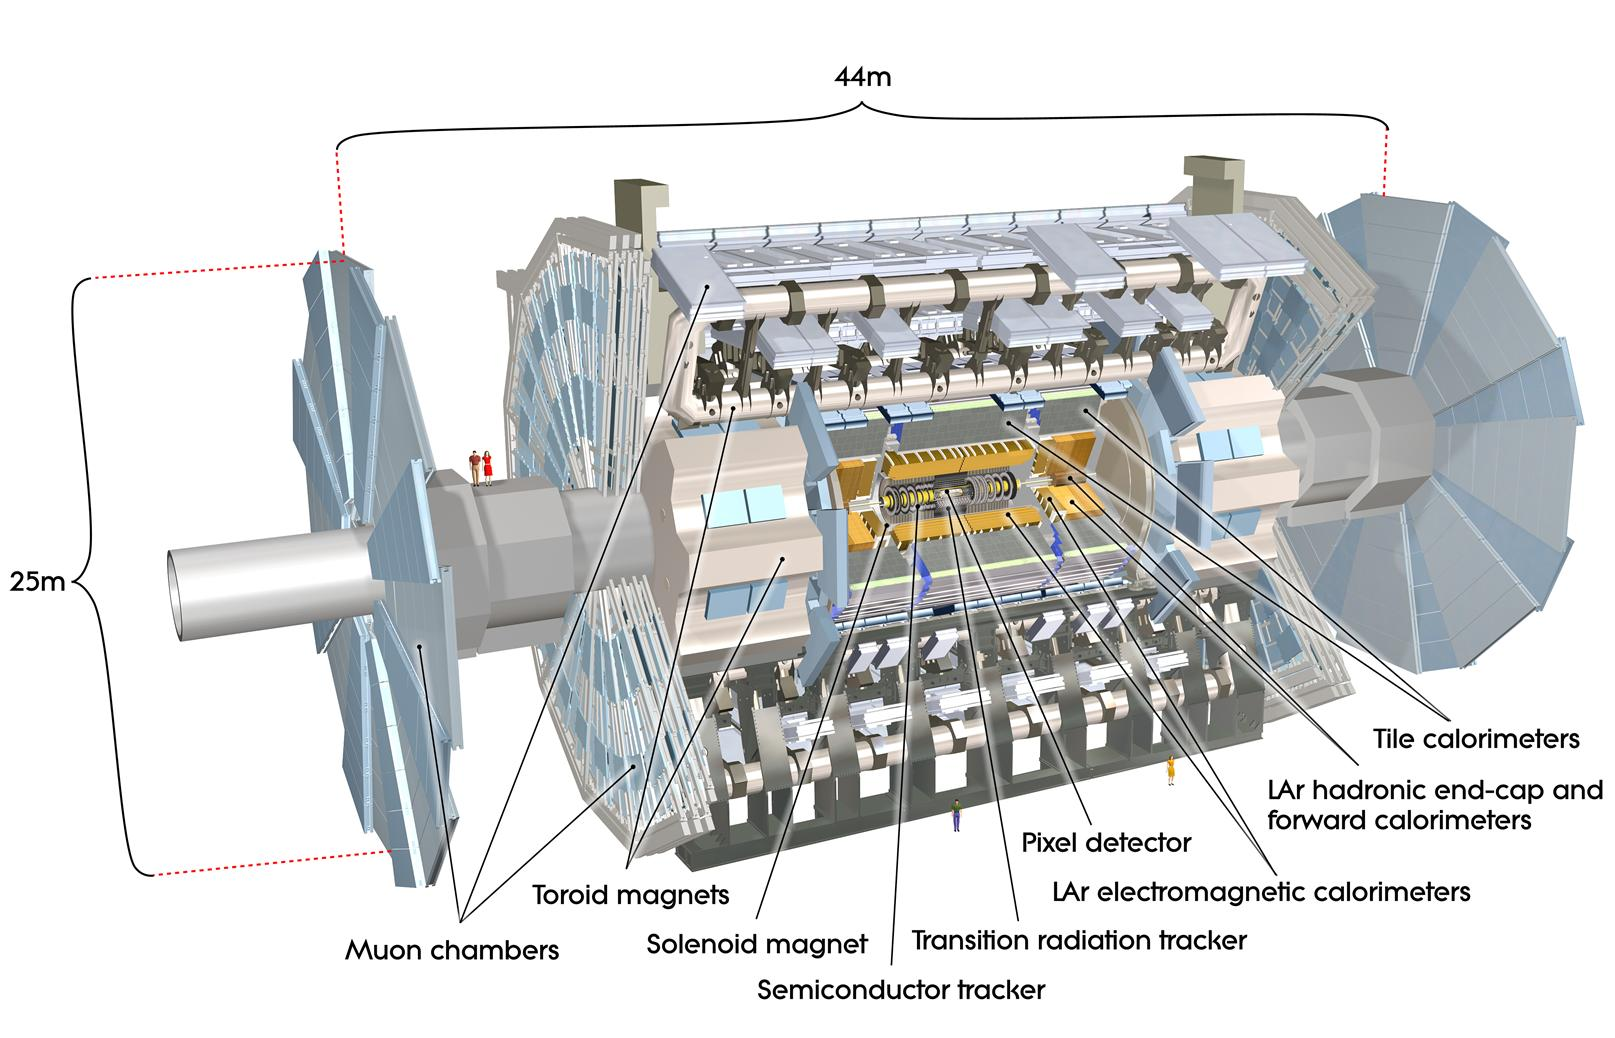
\includegraphics[width=0.9\linewidth]{figures/atlas.jpg}
    \caption{The ATLAS detectors and its components \cite{Pequenao:1095924}}
    \label{fig:atlas-schematic}
\end{figure}

\subsection{The Inner Detector}
\label{subsect:inner-detector}f
Immediately surrounding the interaction point is the Inner Detector, consisting of 3 subsystems constructed from two sensing technologies. These subsystems include a Pixel detector, a Semi-Conductor Tracker (SCT), and a Transition Radiation Tracker (TRT), in the same order of increasing radial distance from the IP. The first two use silicon sensors to detect the passage of a charged particle and the latter a collection of gas-filled straw tube and a tungsten wire to collect the secondary radiation engendered from the particle.

The ID is responsible for precise measurements of discrete points along the path of a charged particle, from which its trajectory (tracks) is reconstructed. Tracks are essential inputs to reconstruct physics objects charged leptons, jets, as well as the identification of jets from heavy quarks. 

A crucial part of the ID's function is the estimation of particle momentum and impact parameters. In the presence of a homogeneous magnetic field of 2T permeating the ID along the $z$-axis, charged particles move in helical orbits, whose radius depends on the transverse momentum $p_T$
\begin{equation}
    \label{eq:3.3}
    R = \frac{p_T}{qB}.
\end{equation}
In principle, by fitting a helix through measurements on a track, one obtains an estimate of the curvature and thus $p_T$. Extrapolating this helix to the point of closest approach to the IP, called the \textit{perigee}, one obtains an estimate of the primary and longitudinal impact parameters $(d_0, z_0)$ respectively. This procedure is described in detail in chapter \ref{chap:atlas-reco-chain}. 

Being the first sub-detector to observe particles after they are created in the entire detector, the ID has the best position to characterize their kinematics to the highest possible resolution. In particular, the relative momentum resolution $p_T\sigma(\frac{q}{p_T})$ is $O(1\%)$, while the impact parameter resolutions can reach $\sigma(d0)\approx 25\mu m$ and $\sigma(z0)\approx 40\mu m$. This level of resolution is remarkable considering the physical dimensions of ATLAS, which can only be achieved through meticulous custom designs of the subsystems described below.

\subsubsection{The Pixel Detector}
The pixel detector (figure \ref{fig:atlas-pixel}) is the innermost part of the ID, consisting of 3 barrel layers extending from a radius of $r=50.5\, mm$ up to $r=122.5\, mm$, and 3 end-cap disks on each sides of the barrel. These physical layers each provide a structure onto which detector modules are mounted. Each barrel layer consists of supporting staves  from pixel modules mounted on supporting staves, and each end-cap from 8 sectors circularly arranged around the $z$-axis, each containing 6 modules. In total, the pixel detector has 1744 identical modules, each composed of an array of silicon sensor and 16 front-end chips which read out the electrical signal created by the passage of a charge particle. \cite{front-end-chips} 

A sensor element is fabricated from a detector-grade n-type silicon wafer implanted with high positive ($p^+$) and negative ($n^+$) dose regions on each side. At the $p^+$-$n$ junction, holes from the $p^+$ region neutralize free electrons in the $n$-typed bulk, creating a depletion zone devoid of free charge carriers. Operated in a reverse bias, this region is enlarged over the whole sensor bulk volume. Although containing no free charge carrier, the $pn$-junction is easily ionized by a traversing particle, creating electron-hole pairs. Primary electrons, those directly created by the traversing particle, are often energetic enough to induce secondary ionization and amplify the signal. Electron-hole pairs are separated by the biasing electric field and drift toward their corresponding electrodes. As electrons approach the anode, they are multiplied and measured by the read-out chips.

The sensitive part of a pixel module is approximately $2\times 6\,cm^2$ in size, segmented into highly granular pixels of dimensions $50\times 400 \, \mu m^2$, totalling 47268 pixels. Nearly every pixel corresponds to a readout channel, providing the pixel detector approximately 80 million channels. With the inclusion of the Insertable B-Layer (IBL), the total number of channels the smallest pixel dimension is reduced to $50\times 250$ $\mu m^2$, and the total number of readout channels increased to $94$ million. This high level of granularity enables high precision measurements very close to the beam pipe. The eta

\begin{figure}[h!]
     \centering
     \begin{subfigure}[b]{0.49\textwidth}
         \centering
         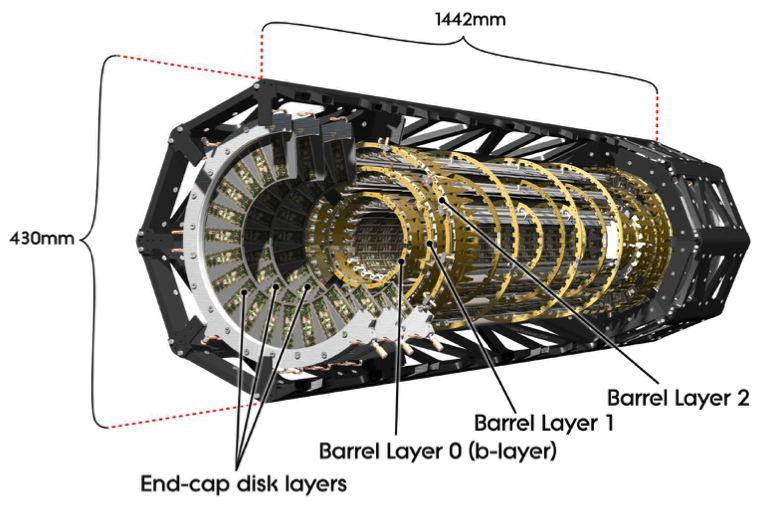
\includegraphics[width=\textwidth]{figures/pixel-detector.png}
         \caption{The ATLAS pixel detector}
         \label{fig:atlas-pixel}
     \end{subfigure}
     \hfill
     \begin{subfigure}[b]{0.49\textwidth}
         \centering
         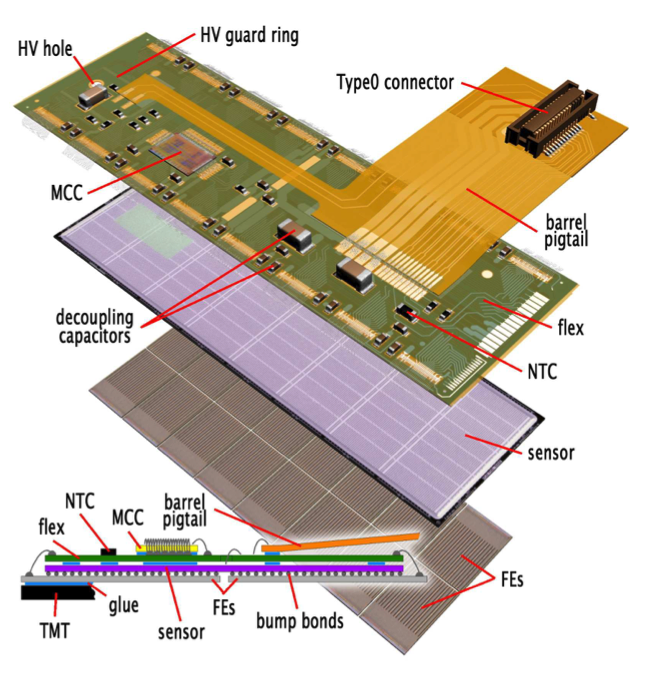
\includegraphics[width=\textwidth]{figures/pixel-module.png}
         \caption{The pixel detector module}
         \label{fig:pixel-module}
     \end{subfigure}
    \caption{The ATLAS pixel detector and detector module. Figures taken from reference~\cite{ID-pixel}}
    \label{fig:pixel-detector-and-module}
\end{figure}

\subsubsection{The Semi-Conductor Tracker}

Surrounding the Pixel volume is the Semi-Conductor Tracker (SCT), consisting of four barrel layers and eighteen symmetric end-cap disks, both featuring a total of 4088 strip modules \cite{ATLAS-TDR-04, ATLAS-TDR-05}. Figure \ref{subfig:strip-module} provides an overview of a strip module used in the barrel layers. Each detector module consists of two pairs of single-sided microstrips with $80$ $\mu m$ pitch. Each single strip sensor is capable of detecting particle intersection in one dimension, information from a pair of strips must be combined to provide three-dimensional point information with space-point resolution of 16 $\mu m$ in the $(R-\phi)$ direction and 580 $\mu m$ in the $z$-direction \cite{BARONE201357}. 

\begin{figure}[h!]
     \centering
     \begin{subfigure}{0.7\textwidth}
         \centering
         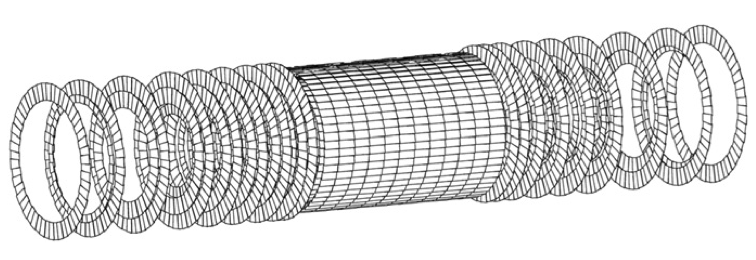
\includegraphics[width=\textwidth]{figures/sct-detector.png}
         \caption{The ATLAS pixel detector}
         \label{subfig:sct-detector}
     \end{subfigure}
     % \hfill
     \begin{subfigure}{0.65\textwidth}
         \centering
         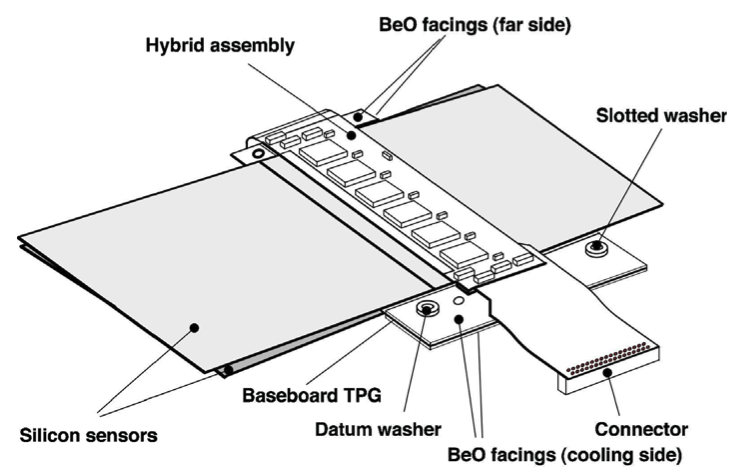
\includegraphics[width=0.9\textwidth]{figures/strip-module.png}
         \caption{The pixel detector module}
         \label{subfig:strip-module}
     \end{subfigure}
    \caption{Overview of the strip module of the SCT in the barrel layers. Figures taken from reference~\cite{Robinson_2013}}
    \label{fig:sct-detector}
\end{figure}

% \begin{figure}[h!]
%     \centering
%     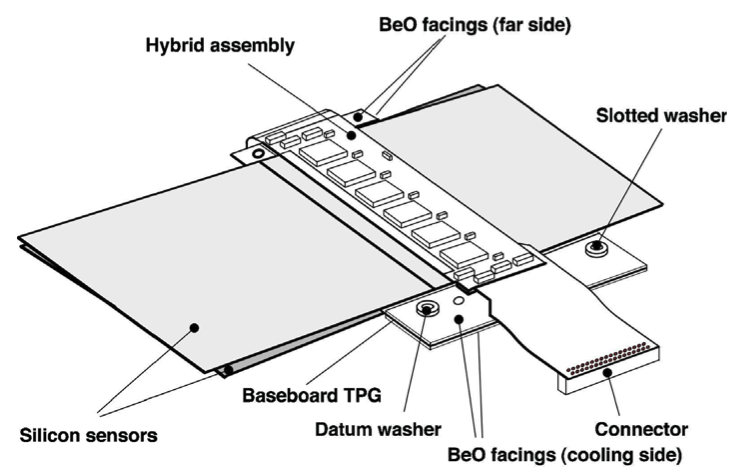
\includegraphics[width=0.5\linewidth]{figures/strip-module.png}
%     \caption{Overview of the strip module of the SCT in the barrel layers}
%     \label{fig:strip-module}
% \end{figure}

\subsubsection{The Transition Radiation Tracker}
The Transition Radiation Tracker (TRT) is the outermost component of the Inner Detector. It comprises of approximately 300000 straw tubes that are 4 $mm$ in diameter, and covers up to $\abs{\eta}=1$ in the barrel and $\abs{\eta} =2$ in the end-cap layers. Each high $p_T$ track passing through the TRT leaves $30-36$ hits and reach a resolution of 130 $\mu m$ in the $(R-\phi)$ direction. 

In each straw tube, a tungsten wire is located at the center and surrounded by a gas mixture spreading the volume of the tube. When a charged particle passes through the tube, it ionizes the ambient gas and creates an pairs of electrons and positive gas ions. An electric field exists between the outer tube and the central wire, which now act as electrodes, separating the charges. As they reach the wire, the charges are amplified and detected. To enhance electron identification, the straw tubes are surrounded by polymer fibers (barrel) and foils (end-caps), which facilitate transition radiation at the interface between materials. 

\subsection{The Calorimeter system}

The second group of detector subsystems, the calorimeters, is dedicated to the measurement of particle energies and directions. There exist two types of calorimeters: electromagnetic and hadronic. 
They detect particle through alternating layers of passive and active materials. 
In the passive layers, also called the absorber, an energetic particle deposits a large portion of its kinetic energy and induces a large number of secondary particles, including electrons, photons, and hadrons, depending on the type of calorimeter. 
These particles are then stopped and measured by the active layers. 

The electromagnetic calorimeter targets electrons/positrons and photons, which create electromagnetic showers as they interact with the inactive material. In the electric field near the atomic nuclei that make up the material, electrons and position undergo Brehmsstrahlung and emit secondary photons, which induces electron pair production in the vicinity of atomic nuclei and generates more high-energy charged particles. 
A reaction chain in which Brehmsstrahlung photons induce electrons/positrons, which emits more Brehmsstrahlung photons, creates a shower of charged particles in the passive material. 

In the case of the hadronic calorimeters, hadrons passing through a dense material interact with its nuclei and produce secondary hadrons, mostly pions, which then drives the reaction chain, similar to the electromagnetic counterpart. In addition, neutral pion decays to high-energy photon and leptonic decays can also induce electromagnetic subshower within a hadronic shower. 

\subsubsection{The electromagnetic (EM) calorimeter}
The passive absorber material in the ATLAS electromagnetic calorimeter comprises of lead, and the active material of liquid argon. The passive layers are interspersed with active layers in an accordion pattern. The barrel covers a pseudoscalar range up to $\abs{\eta} = 1.475$ and the endcaps $1.375 < \abs{\eta}<3.2$. The central region of the EM calorimeter consists of three layers and a pre-sampler with a fine granularity $(\eta\times\phi=0.025\times 0.1)$. The first sampling layer features a segmentation of $\eta\times\phi=0.025/8\times 0.1$, while the second and third sampling layers are segmented into $\eta\times\phi=0.025\times 0.025$ and $\eta\times\phi=0.025\times 0.05$, respectively. Angular segmentation allows measurements of particle directions, and depth segmentation measurements of shape. This information is in turn useful in discriminating electrons and photons from jets. Figure \ref{subfig:em-calorimeter-module} shows a sketch of the EM calorimeter module in the barrel. 

\begin{figure}[h!]
    \begin{subfigure}[b]{0.59\textwidth}
    \centering
    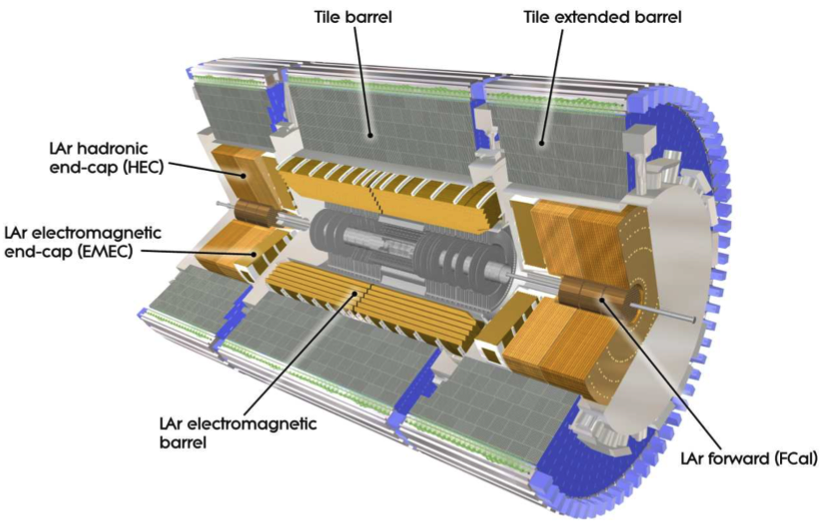
\includegraphics[width=\textwidth]{figures/calorimeter-system.png}
    \caption{}
    \label{subfig:calorimeter-system}
    \end{subfigure}
    \hfill
    \begin{subfigure}[b]{0.4\textwidth}
    \centering
    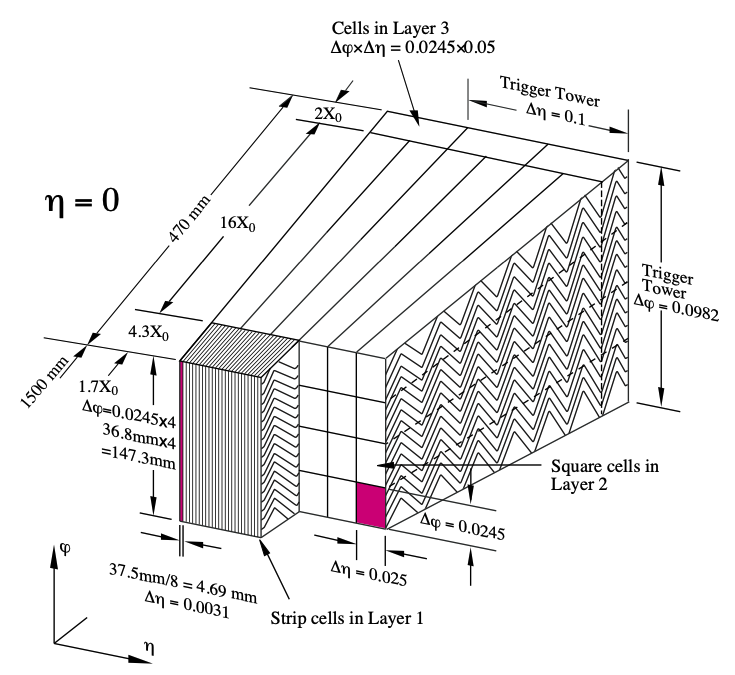
\includegraphics[width=\textwidth]{figures/Em-calorimeter.png}
    \caption{}
    \label{subfig:em-calorimeter-module}
    \end{subfigure}
    \caption{(a) Layout of the ATLAS calorimetry system, and (b) sketch of a barrel module of the electromagnetic calorimeter~\cite{atlas_exp_2008}.}
    \label{fig:calorimeter}
\end{figure}

\subsubsection{The hadronic calorimeter}
The hadronic calorimeter uses iron absorbers and plastic scintillating tiles as active material in the barrel region. It covers a pseudorapidity range of $\abs{\eta} < 1.0$ in the barrel and $0.7 < \abs{\eta} < 1.7$ in the extended barrel. It also comprises of three layers of increasing radii. The effective granularity varies between $\eta\times\phi=0.1\times 0.1$ and $0.2\times 0.1$. 

The endcap and forward regions (figure \ref{subfig:calorimeter-system}) of the hadronic calorimeter uses copper/tungsten as absorber and liquid Argon as active material. They cover a pseudorapidity range of up to 4.9. The forward calorimeter is split into an electromagnetic and a hadronic component. 

\subsection{The muon spectrometer}
Unlike other particles, muons produced with energy in the range of $0.1-100$ GeV typically seen in ATLAS do not strongly interact with detector material in the detector subsystems described in the previous sections. Despite leaving energy clusters in the ID, they traverse the calorimeters intact are therefore measured by a dedicated muon system. The muon spectrometer is composed of four subsystems that use different technologies to 
track muon at high precision and perform fast triggers. It is immersed in a toroidal magnetic field ranging from 2.0 to 6.0 T, providing enough bending power to resolve the muon transverse momentum. Figure \ref{fig:MS-system} shows the overall layout of and a side view of a quadrant of the MS, including its subsystems. 

\begin{figure}[h!]
    \begin{subfigure}[b]{0.4\textwidth}
    \centering
    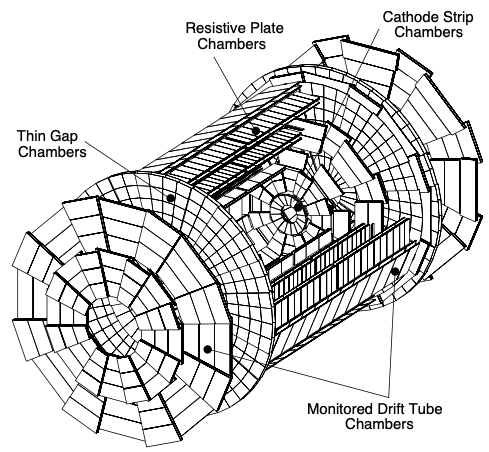
\includegraphics[width=\textwidth]{figures/MS-overview.png}
    \caption{}
    \label{subfig:MS-system-overview}
    \end{subfigure}
    \hfill
    \begin{subfigure}[b]{0.59\textwidth}
    \centering
    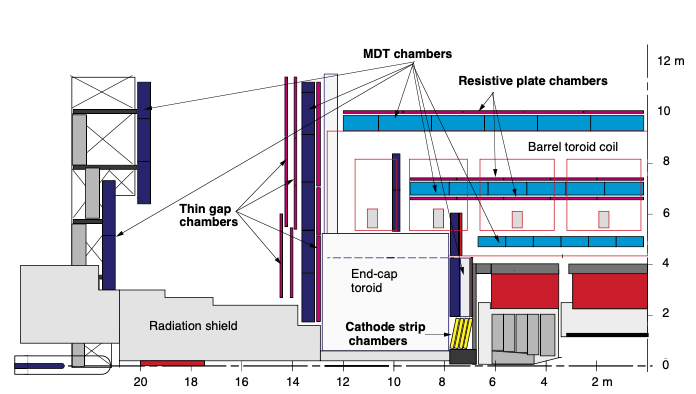
\includegraphics[width=\textwidth]{figures/MS-sideview.png}
    \caption{}
    \label{subfig:MS-system-sideview}
    \end{subfigure}
    \caption{(a) Layout of the ATLAS Muon Spectrometer system, and (b) a sideview of one quadrant of the MS~\cite{ATLAS-TDR-10}.}
    \label{fig:MS-system}
\end{figure}

To measure the curvature of muon tracks along the bending direction of the toroidal field, the MS uses a number of aluminum tubes of 30 milimeters in diameter filled with Ar and having a central tungsten/rhenium alloy wire, similar to the TRT. The outer surface and the central wire of these Monitored Drift Tubes (MDTs) are kept at a potential difference of 3 kV to ensure a drifting time of less than 700 ns. The MDTs are divided into 1200 chambers cover a pseudorapidity range up to $\abs{\eta} =2.7$, each chamber providing 6 to 8 measurements along the track.

At larger $\abs{\eta}$, the Cathode Strip Chambers (CSCs) have a higher granularity than the MDTs to resolve large backgrounds in the forward region. They cover $2.0< \abs{\eta} < 2.7$ and have short drift times of around $40$ ns. The CSCs provide 4 simultaneous measurements of $\eta$ and $\phi$.

The Resistive Plate Chambers (RPCs), used in the barrel and the Thin Gap Chambers (TGCs), used in the endcap regions are both gaseous detectors and together make up the muon trigger system. They respectively cover $\abs{\eta} < 1.05$ and $1.05 < \abs{\eta} < 2.4$.

% \subsection{The magnet system}

% \subsection{Trigger and Data Acquisition System}

% \section{Summary}
